\section{Getting started}
\begin{frame}[fragile]
  \slidetitle

  This section covers the following topics:
  \begin{itemize}
    \item Configure git
    \item Obtain a git repository
    \item Add files
    \item Stage changes
    \item Commit changes
    \item The git work flow
    \item Undo modifications and staging
  \end{itemize}
\end{frame}

\subsection{Configuring git}
\begin{frame}[fragile]
  \subslidetitle
  Many useful features can be configured with git:
  \begin{itemize}
    \item User settings
    \item Colored output
    \item Command aliases
    \item Tools to be used
  \end{itemize}

  \vspace{1em}
  The minimum configuration needs your name and email address.\\
  Let's configure this by using the \cmd{git config} command:
  \begin{lstlisting}
$ (*\textcolor[HTML]{0000AA}{git config --global user.name "My name"}*)
$ (*\textcolor[HTML]{0000AA}{git config --global user.email "myemail@address"}*)
\end{lstlisting}

  \vspace{1em}
  Note: The global git configuration is stored in \cmd{\textasciitilde/.gitconfig}.

\end{frame}

\subsection{Obtaining a repository}
\begin{frame}[fragile]
  \subslidetitle
  A git repository can be obtained only by downloading a whole git repository,
  called a working copy.
  \\
  \vspace{1em}
  Let's clone the gitmoon repository by using \cmd{git clone}:
  \begin{lstlisting}
$ (*\textcolor[HTML]{0000AA}{git clone https://github.com/neolynx/gitmoon.git}*)
Cloning into 'gitmoon'...
remote: Counting objects: 6, done.
remote: Compressing objects: 100% (6/6), done.
remote: Total 6 (delta 0), reused 6 (delta 0), pack-reused 0
Unpacking objects: 100% (6/6), done.
Checking connectivity... done.
\end{lstlisting}

  \vspace{1em}
  Note: a new repository can be created with the \cmd{git init} command.
\end{frame}

\subsection{Workshop git project}
\begin{frame}[fragile]
  \subslidetitle
  Let's see what we find in the working copy:
  \begin{lstlisting}
$ (*\textcolor[HTML]{0000AA}{cd gitmoon}*)
$ (*\textcolor[HTML]{0000AA}{ls}*)
moon_1024.jpg  moon.html  moon.js  three.min.js
\end{lstlisting}

  \vspace{1em}
  Oh, there is a HTML file !
  \begin{lstlisting}
$ (*\textcolor[HTML]{0000AA}{firefox moon.html \&}*)
\end{lstlisting}
\end{frame}

\subsection{Checking the status}
\begin{frame}[fragile]
  \subslidetitle

  The command \cmd{git status} shows the state of the local working copy:
  \begin{lstlisting}
$ (*\textcolor[HTML]{0000AA}{git status}*)
On branch master
Your branch is up-to-date with 'origin/master'.
nothing to commit, working directory clean
\end{lstlisting}
\end{frame}

\subsection{Create .gitignore}
\begin{frame}[fragile]
  \subslidetitle
  The .gitignore file contains a list of files git should ignore. For example temporary file, generated output you name it!

  \vspace{1em}
  Let's create a .gitignore file ignoring temporary vim swp files:
  \begin{lstlisting}
$ (*\textcolor[HTML]{0000AA}{echo '*.swp' > .gitignore}*)
\end{lstlisting}

  \vspace{1em}
  Note: use wildcard patterns to generalize your ignore list. The root .gitignore file applies to all sub folders.

\end{frame}

\subsection{Our first commit}
\begin{frame}[fragile]
  \subslidetitle

  The combination of \cmd{git add} and \cmd{git commit} commands create a git commit of the .gitignore file:
  \begin{lstlisting}
$ (*\textcolor[HTML]{0000AA}{git add .gitignore}*)
$ (*\textcolor[HTML]{0000AA}{git commit -m "add .gitignore file"}*)
[master 8334b05] add .gitignore file
 1 file changed, 1 insertion(+)
 create mode 100644 .gitignore
\end{lstlisting}

Not so difficult!? Let's explain it step by step in the following slides.
\end{frame}

\subsection{Adding a file}
\begin{frame}[fragile]
  \subslidetitle

  Let's create an AUTHORS file with your name:
  \begin{lstlisting}
$ (*\textcolor[HTML]{0000AA}{echo Tux Penguin > AUTHORS}*)
\end{lstlisting}

  Check the git status:
  \begin{lstlisting}
$ (*\textcolor[HTML]{0000AA}{git status}*)
On branch master
Your branch is ahead of 'origin/master' by 1 commit.
  (use "git push" to publish your local commits)
Untracked files:
  (use "git add <file>..." to include in what will be committed)

        (*\textcolor[HTML]{AA0000}{AUTHORS}*)

nothing added to commit but untracked files present (use "git add" to track)
\end{lstlisting}

\end{frame}

\subsection{Adding a file}
\begin{frame}[fragile]
  \subslidetitle

  The command \cmd{git add} tells git to track the file:
  \begin{lstlisting}
$ (*\textcolor[HTML]{0000AA}{git add AUTHORS}*)
\end{lstlisting}

  Check the git status:
  \begin{lstlisting}
$ (*\textcolor[HTML]{0000AA}{git status}*)
On branch master
Your branch is ahead of 'origin/master' by 1 commit.
  (use "git push" to publish your local commits)
Changes to be committed:
  (use "git reset HEAD <file>..." to unstage)

        (*\textcolor[HTML]{00AA00}{new file:}*)   (*\textcolor[HTML]{00AA00}{AUTHORS}*)
\end{lstlisting}

  \vspace{1em}
  Note: only files can be tracked, git treats directories as part of the file name
\end{frame}


\subsection{Creating a commit}
\begin{frame}[fragile]
  \subslidetitle

  The command \cmd{git commit} tells git to commit the file:
  \begin{lstlisting}
$ (*\textcolor[HTML]{0000AA}{git commit -m "add authors file"}*)

[master c01af7f] add authors file
 1 file changed, 1 insertion(+)
 create mode 100644 AUTHORS
\end{lstlisting}

  Check the git status:
  \begin{lstlisting}
$ (*\textcolor[HTML]{0000AA}{git status}*)
On branch master
Your branch is ahead of 'origin/master' by 2 commit.
  (use "git push" to publish your local commits)
nothing to commit, working directory clean
\end{lstlisting}
\end{frame}

\subsection{Git workflow}
\begin{frame}[fragile]
  \subslidetitle
  The following diagram illustrates the workflow we just did: \\
  \vspace{2em}
  \centerline{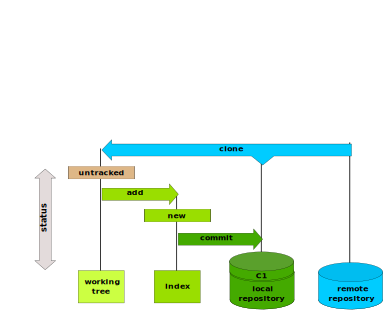
\includegraphics{diagrams/getting_started.pdf}}

  \vspace{1em}
  Note: the \textbf{index} is also called \textbf{staging area}
\end{frame}


\subsection{Modifying a file}
\begin{frame}[fragile]
  \subslidetitle

  Let's change the \cmd{<title>} tag to 'Git Moons' in the \cmd{moon.html} file

  Check the git status:
  \begin{lstlisting}
$ (*\textcolor[HTML]{0000AA}{git status}*)
On branch master
Your branch is up-to-date with 'origin/master'.
Changes not staged for commit:
  (use "git add <file>..." to update what will be committed)
  (use "git checkout -- <file>..." to discard changes in working directory)

        (*\textcolor[HTML]{AA0000}{modified:}*)   (*\textcolor[HTML]{AA0000}{moon.html}*)

no changes added to commit (use "git add" and/or "git commit -a")
\end{lstlisting}
\end{frame}

\subsection{Showing changes}
\begin{frame}[fragile]
  \subslidetitle

  The command \cmd{git diff} show the difference between working tree and index:
  \begin{lstlisting}
$ (*\textcolor[HTML]{0000AA}{git diff}*)
diff --git a/moon.html b/moon.html
index d344c62..22e0c8e 100644
--- a/moon.html
+++ b/moon.html
(*\textcolor[HTML]{0000EE}{@@ -1,7 +1,7 @@}*)
 <!DOCTYPE html>
 <html>
     <head>
(*\textcolor[HTML]{AA0000}{-}*)        (*\textcolor[HTML]{AA0000}{<title>moon</title>}*)
(*\textcolor[HTML]{00AA00}{+}*)        (*\textcolor[HTML]{00AA00}{<title>Git Moons</title>}*)
         <meta charset="utf-8">
\end{lstlisting}
\end{frame}

\subsection{Staging modifications}
\begin{frame}[fragile]
  \subslidetitle

  The command \cmd{git add} tells git to stage the modifications:
  \begin{lstlisting}
$ (*\textcolor[HTML]{0000AA}{git add moon.html}*)
\end{lstlisting}

  Check the git status:
  \begin{lstlisting}
$ (*\textcolor[HTML]{0000AA}{git status}*)
On branch master
Your branch is ahead of 'origin/master' by 2 commit.
  (use "git push" to publish your local commits)
Changes to be committed:
  (use "git reset HEAD <file>..." to unstage)

        (*\textcolor[HTML]{00AA00}{modified:}*)   (*\textcolor[HTML]{00AA00}{moon.html}*)
\end{lstlisting}
  \vspace{1em}
  Note: We stage modifications to make them ready to commit
\end{frame}

\subsection{Committing staged changes}
\begin{frame}[fragile]
  \subslidetitle

  The command \cmd{git commit} tells git to commit the index (staging area) to the local repository:
  \begin{lstlisting}
$ (*\textcolor[HTML]{0000AA}{git commit -m "change title"}*)
[master fc92204] change title
 1 file changed, 1 insertion(+), 1 deletion(-)
\end{lstlisting}
\end{frame}

\subsection{Git workflow}
\begin{frame}[fragile]
  \subslidetitle
  The following diagram illustrates the workflow we just did: \\
  \vspace{2em}
  \centerline{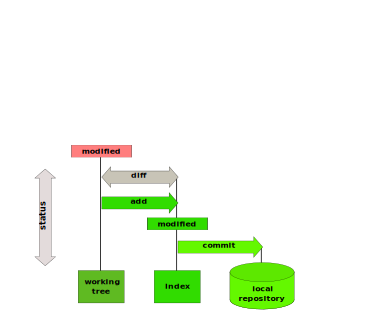
\includegraphics{diagrams/diff-modified-add-commit.pdf}}
\end{frame}

\subsection{Undoing a modification}
\begin{frame}[fragile]
\subslidetitle

  Let's modify a file and verify the git status:
  \begin{lstlisting}
$ (*\textcolor[HTML]{0000AA}{echo "Tux le Pinguin" >> AUTHORS}*)
$ (*\textcolor[HTML]{0000AA}{git status}*)
On branch master
Your branch is ahead of 'origin/master' by 3 commits.
  (use "git push" to publish your local commits)
Changes not staged for commit:
  (use "git add <file>..." to update what will be committed)
  (use "git checkout -- <file>..." to discard changes in working directory)

        (*\textcolor[HTML]{AA0000}{modified:}*)   (*\textcolor[HTML]{AA0000}{AUTHORS}*)

\end{lstlisting}

\end{frame}

\subsection{Undoing a modification}
\begin{frame}[fragile]
\subslidetitle
  The command \cmd{git checkout} allows you to undo the modification:
  \begin{lstlisting}
$ (*\textcolor[HTML]{0000AA}{git checkout AUTHORS}*)
$ (*\textcolor[HTML]{0000AA}{git status}*)
On branch master
Your branch is ahead of 'origin/master' by 3 commits.
  (use "git push" to publish your local commits)
nothing to commit, working directory clean
\end{lstlisting}

  \vspace{1em}
  \centerline{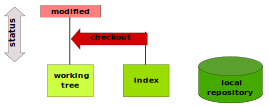
\includegraphics{diagrams/undo-modified}}

  \vspace{1em}
  Note: checkout discards the changes, handle with care!
\end{frame}

\subsection{Unstaging modifications}
\begin{frame}[fragile]
\subslidetitle

  Let's modify a file and stage it:

\begin{lstlisting}
$ (*\textcolor[HTML]{0000AA}{echo "Tux le Pinguin" >> AUTHORS}*)
$ (*\textcolor[HTML]{0000AA}{git add AUTHORS}*)
$ (*\textcolor[HTML]{0000AA}{git status}*)
On branch master
Your branch is ahead of 'origin/master' by 3 commits.
  (use "git push" to publish your local commits)
Changes to be committed:
  (use "git reset HEAD <file>..." to unstage)

        (*\textcolor[HTML]{00AA00}{modified:}*)   (*\textcolor[HTML]{00AA00}{AUTHORS}*)
\end{lstlisting}

\end{frame}

\subsection{Unstaging modifications}
\begin{frame}[fragile]
\subslidetitle

  The command \cmd{git reset} allows you to unstage a file:

  \begin{lstlisting}
$ (*\textcolor[HTML]{0000AA}{git reset AUTHORS}*)
Unstaged changes after reset:
M       AUTHORS
\end{lstlisting}

  \vspace{1em}
  \centerline{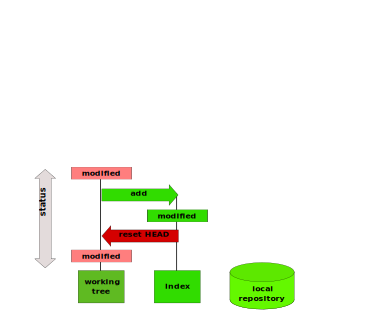
\includegraphics{diagrams/undo-staged}}
\end{frame}


\subsection{Resetting modifications}
\begin{frame}[fragile]
\subslidetitle
  After \cmd{git reset}, the modification is still there:
\begin{lstlisting}
$ (*\textcolor[HTML]{0000AA}{git status}*)
On branch master
Your branch is ahead of 'origin/master' by 3 commits.
  (use "git push" to publish your local commits)
Changes not staged for commit:
  (use "git add <file>..." to update what will be committed)
  (use "git checkout -- <file>..." to discard changes in working directory)

        (*\textcolor[HTML]{AA0000}{modified:}*)   (*\textcolor[HTML]{AA0000}{AUTHORS}*)
\end{lstlisting}

  Instead of using \cmd{git checkout} on each file, \\
  use \cmd{git reset --hard} to reset all modifications at once:
\begin{lstlisting}
$ (*\textcolor[HTML]{0000AA}{git reset --hard}*)
HEAD is now at fc92204 change title
\end{lstlisting}
\end{frame}

\subsection{Removing a file}
\begin{frame}[fragile]
\subslidetitle
  Let's first create a file and commit it:
\begin{lstlisting}
$ (*\textcolor[HTML]{0000AA}{touch test.file}*)
$ (*\textcolor[HTML]{0000AA}{git add test.file}*)
$ (*\textcolor[HTML]{0000AA}{git commit -m "adding a test file"}*)
[master 3d0539f] add test file
 1 file changed, 0 insertions(+), 0 deletions(-)
 create mode 100644 test.file
\end{lstlisting}
\end{frame}

\subsection{Removing a file}
\begin{frame}[fragile]
\subslidetitle
  The command \cmd{git rm} removes a file from the repository:
\begin{lstlisting}
$ (*\textcolor[HTML]{0000AA}{git rm test.file}*)
rm 'test.file'
$ (*\textcolor[HTML]{0000AA}{git status}*)
On branch master
Your branch is ahead of 'origin/master' by 4 commit.
  (use "git push" to publish your local commits)
Changes to be committed:
  (use "git reset HEAD <file>..." to unstage)

        (*\textcolor[HTML]{00AA00}{deleted:}*)    (*\textcolor[HTML]{00AA00}{test.file}*)
\end{lstlisting}

  Commit the staged removal of the file:
  \begin{lstlisting}
$ (*\textcolor[HTML]{0000AA}{git commit -m "we do not need the test file anymore"}*)
[master 06cb00f] remove test file
 1 file changed, 0 insertions(+), 0 deletions(-)
 delete mode 100644 test.file
\end{lstlisting}

\end{frame}

\subsection{Exercises}
\begin{frame}[fragile]
\subslidetitle
  Create a commit for each exercise below:
  \begin{exercise}
    \item Change the color of the moon to blue and\\
      commit as 'blue moon' in \cmd{moon.js}
    \item Change the \cmd{<h1>} tag of \cmd{moon.html} to 'Git Moons' and\\
      commit as 'title in page'
    \item Add a green moon after the blue moon\\
      commit as 'green moon'
  \end{exercise}

\end{frame}

